\clearpage\appendix
\section{Air speed estimation}
\label{airspeedestimation}
Before it is possible to conclude whether the the skirts around the Flatiron building will billow, we first need to know what wind speed is needed to overcome gravity. To estimate this we make use of Bernoulli's principle and a few estimations of the women's skirts.

First off we assume that the wind beneath a woman's skirt is completely standing still when being billowed. Disregarding a difference in height, Bernoulli dictates that the upward force on a woman's skirt is
\begin{equation}
P_2 - P_1 = \frac{\rho_{air}v^2}{2}
\end{equation}
In which $P$ is the pressure, $\rho_{air}$ the density of the air, and $v$ the speed of the wind. The area on which the force can work is under an angle of, assuming, 10 degrees. This makes the effective force on the skirt by the wind
\begin{equation}
F = A \sin{10} \frac{\rho_{air}v^2}{2}
\label{eq:fwind}
\end{equation}
In which $A$ is the area of the skirt. The gravity working on the skirt is defined by a few variables, and can be written as
\begin{equation}
F = g A d \rho_{skirt}
\label{eq:fskirt}
\end{equation}
in which $g$ is the gravitational constant, $d$ the thickness of the skirt, and $\rho_{skirt}$ the density of the skirt. Saying that the forces in \autoref{eq:fwind} and \autoref{eq:fskirt} are equal and then solving for the speed gives
\begin{equation}
v = \sqrt{\frac{2 g d \rho_{skirt}}{\sin{10} \rho_{air}}}
\end{equation}
Filling in the density of air, cotton and 2 mm for the skirt density gives a speed of about 1.3~ms$^{-1}$ to blow up the skirts of women.

\section{Dimensions of the obstacles}
\label{appendixdimensions}
As discussed in \autoref{obstacles}, the obstacles used in the CFD analysis were estimated using Google Maps. In \autoref{maps} it is shown how these distances were estimated. 
\begin{figure}[hb]
\centering
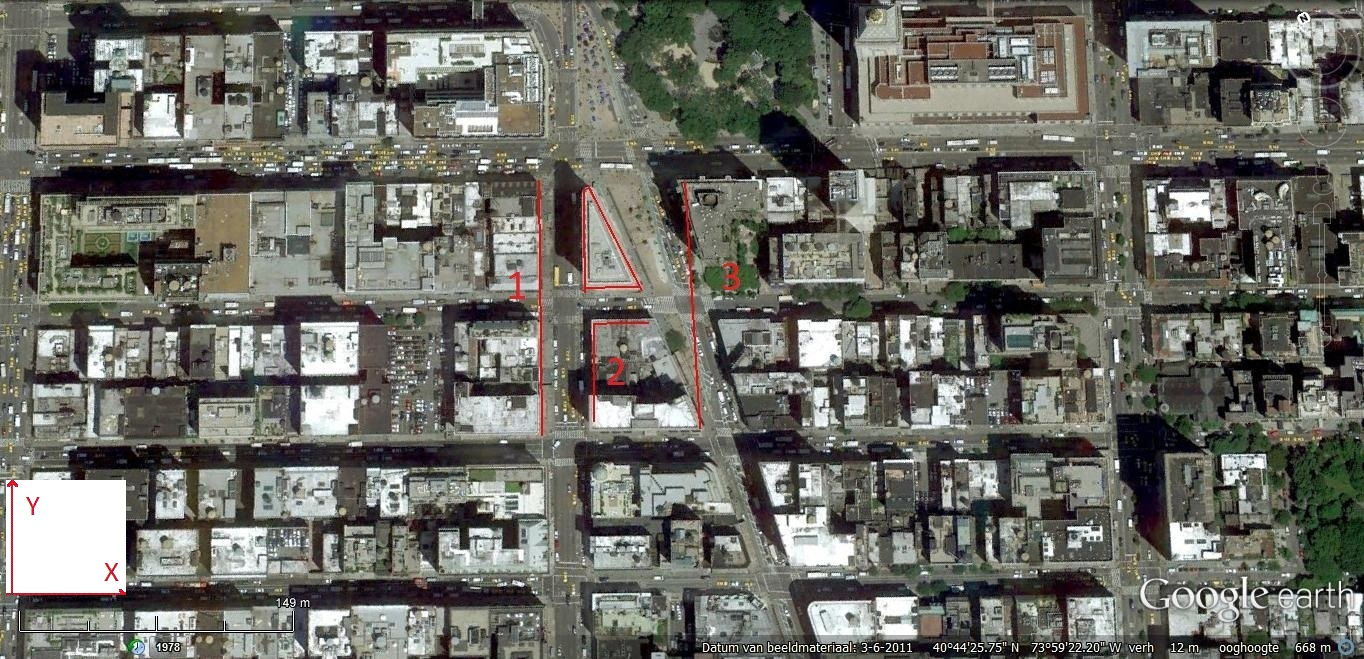
\includegraphics[width = \textwidth]{flatironafschatting.jpg}
\caption{A snapshot of the method used to estimate the dimensions using Google Maps. The red lines indicated the measured distances. }
\label{maps}
\end{figure}
From this figure and the measurement tool on the Google Maps program, we found the following dimensions for the Flatiron building and surroundings. The numbers correspond with the building blocks in \autoref{measurements}. Block number 1 and 3 contain 2 buildings, both exactly the same size and 25 meters apart.

\begin{table}[ht!]
\centering
\caption{Parameters used in the generation of the obstacles that are not the Flatiron building, in meters}
\begin{tabular}{  r  r  r }
\hline
Building block No. & x-length & y-length\\
\hline 
1 & 20 & 60\\
2 & 30 & 60 \\
3 & 20 & 60\\
Space between & 25 & 25 \\
\hline
\end{tabular}
\label{measurements}
\end{table}
%
%
\section{Streamlines}
\label{sec:streamlines}
In this section the streamlines to get a general overview. \\
\begin{figure}[hp]
\centering
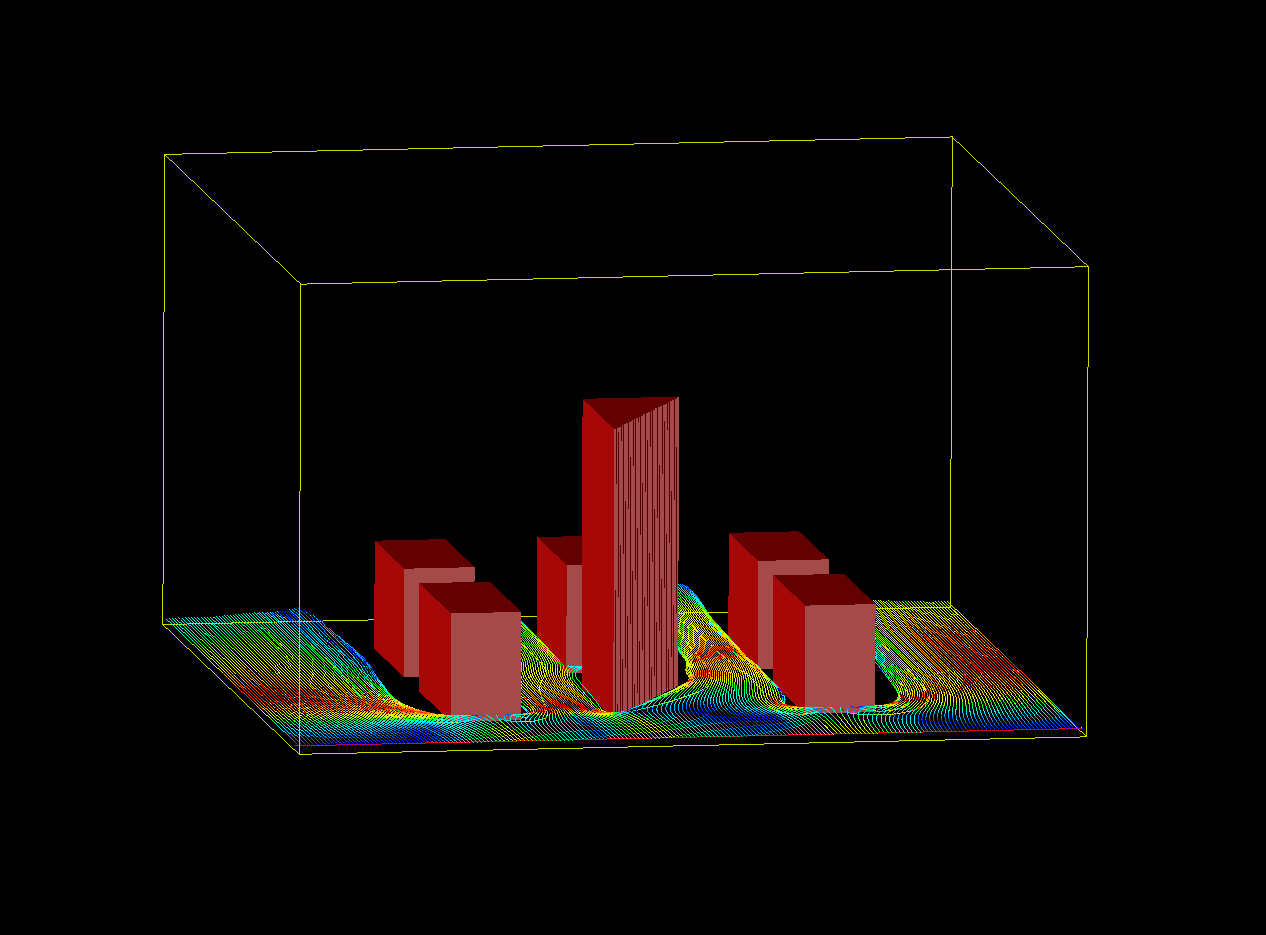
\includegraphics[width =  \textwidth]{streamlinesbottom.png}
\caption{Streamlines around the Flatiron and surrounding buildings just above ground level}
\label{fig:streamlinesbottom}
\end{figure}
\begin{figure}[hp]
\centering
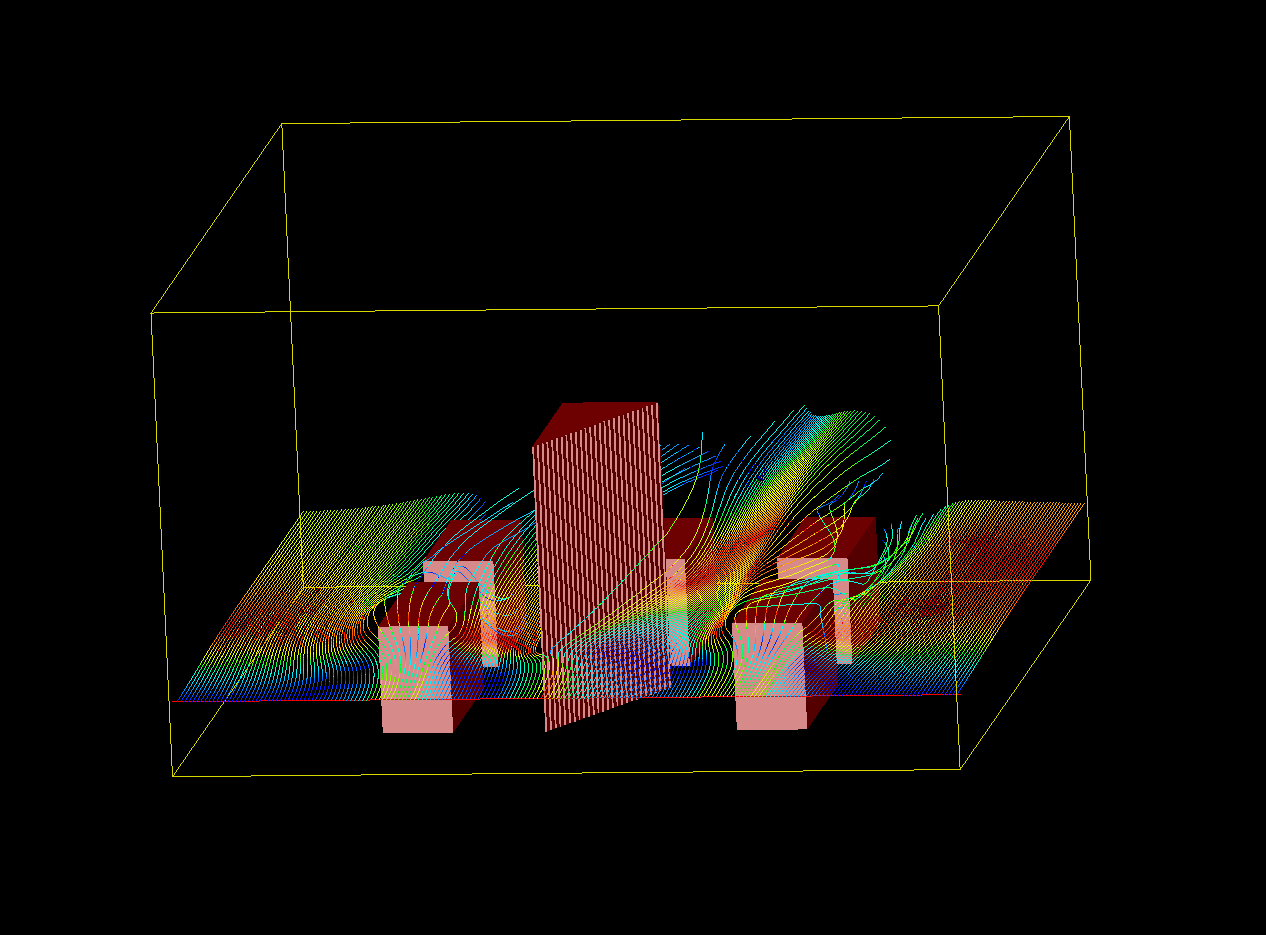
\includegraphics[width = \textwidth]{streamlinesmid.png}
\caption{Streamlines around the Flatiron and surrounding buildings just below the top of the surrounding buildings}
\label{fig:streamlinesmid}
\end{figure}
\begin{figure}[hp]
\centering
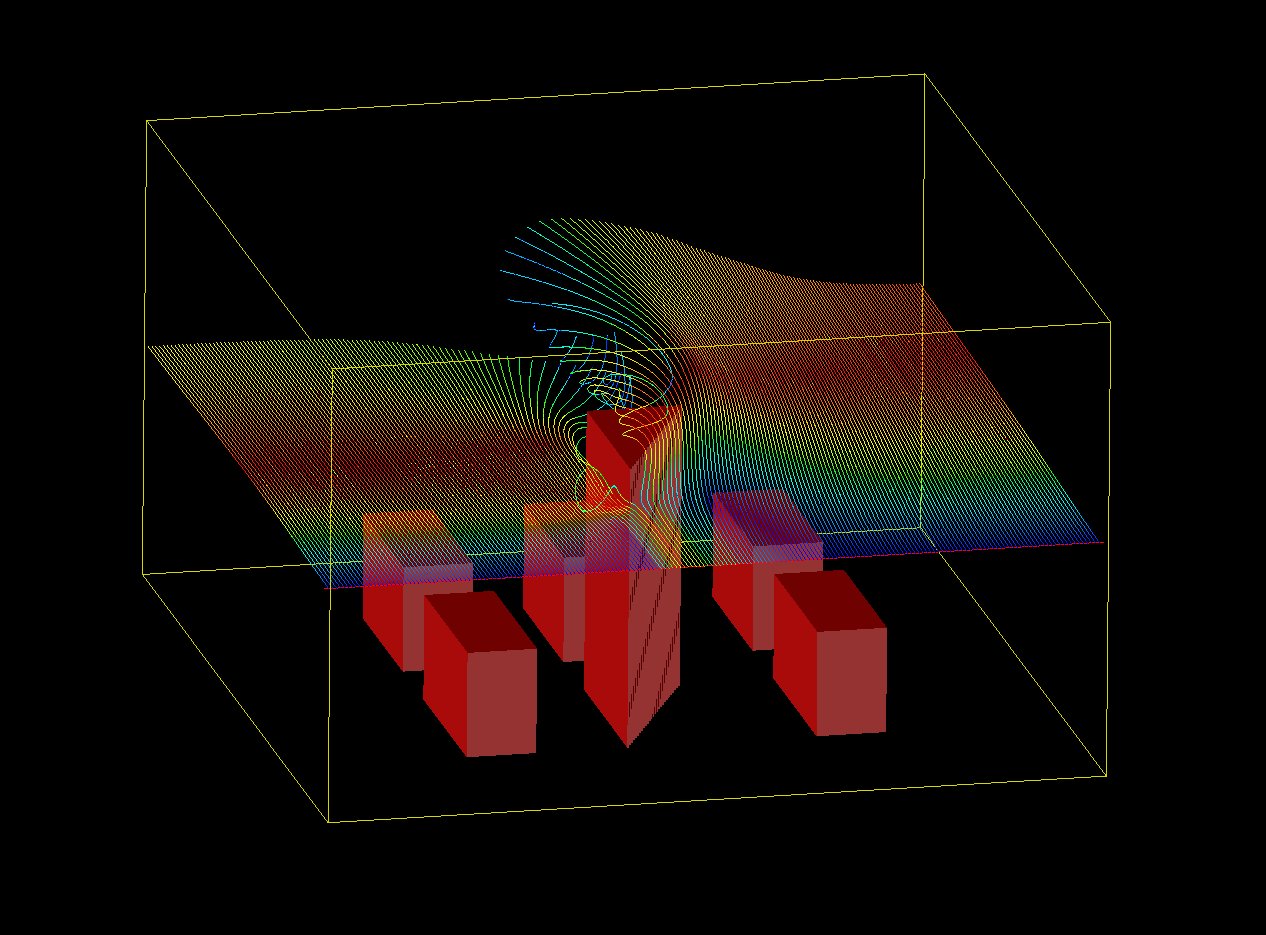
\includegraphics[width = \textwidth]{streamlinestop.png}
\caption{Streamlines around the Flatiron and surrounding buildings just below the top of the Flatiron building}
\label{fig:streamlinestop}
\end{figure}
%
%
\clearpage\section{configuration.yml}
\VerbatimInput{configuration.yml}
